\section{Sistema de observaciones}

Como ya habíamos explicado en el apartado anterior, para obtener las observaciones necesitábamos capturar las imágenes producidas por el juego y enviarlas a los agentes para que entrenaran. La principal dificultad es que el juego y el entorno de \textit{Python} son procesos completamente distintos así que era necesario crear una forma de compartir esta información entre estos procesos.

Planteamos dos alternativas para resolver el problema:

\subsection*{Alternativa 1: Sockets}

La primera alternativa consistía en que al comenzar el juego, conseguir que todo el output visual fuera enviado a través de un socket que estaría conectado con el proceso de \textit{Python}. Para implementar esta comunicación con sockets, ambos procesos deberían crear un thread encargado de la comunicación, además del thread principal. En la Figura \ref {fig:alternativa-1-com} podemos ver un esquema de la arquitectura de esta alternativa.
\begin{figure}[ht]
    \centering
    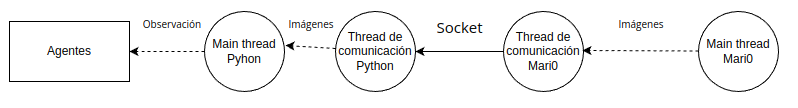
\includegraphics[width=1.0\textwidth]{img/Observations-1.png}
    \caption{Esquema de la alternativa por sockets[Elaboración Propia]}
    \label{fig:alternativa-1-com}
\end{figure}

Esta alternativa tiene diferentes problemas. El problema principal es que realizar el envío de imágenes a través de sockets es un proceso complejo y de programación de bajo nivel. Esto requeriría coordinación entre procesos, decidir cuantas capturas de pantalla se enviarán por segundo para no saturar el canal de comunicación, comunicar los thread de \textit{Python}, modificar casi por completo el renderizado del videojuego, etc.

\subsection*{Alternativa 2: Virtual frame buffer}

La segunda alternativa es usar un Virtual frame buffer para capturar las imágenes del videojuego y luego usar la librería \textit{Mss} \cite {mss} para tomar capturas de este buffer. Esta alternativa es usada en otros proyectos de OpenAI similares como \cite {muphen}. En primer lugar explicaremos que es un Virtual frame buffer.

Un Virtual frame buffer \textit{(Xvfb)} es un servidor de sistema de ventanas que ejecuta todas las operaciones gráficas en memoria sin mostrar nada por pantalla \cite {xvfb-wikipedia}. De forma simple, es un proceso que actúa como una pantalla virtual donde pueden realizarse tareas gráficas como abrir un navegador, jugar a un videojuego, etc. pero sin mostrar ninguna imagen por la pantalla real, todo ocurre en la memoria del ordenador.

El módulo \textit{Mss} es simplemente una librería capaz de tomar capturas de pantalla eficientemente de cualquier display, ya sea un display virtual como en nuestro caso o de la pantalla del ordenador.

Para usar esta tecnología, deberíamos seguir el siguiente proceso. El proceso de \textit{Python} debería crear el proceso del virtual buffer \textit{(Xvfb)} y más tarde el proceso de \textit{Mari0}, que usará el \textit{Xvfb} para renderizar el juego. Finalmente, cuando sea necesario obtener una observación del entorno, el módulo \textit{Mss} se encargará de obtener una captura de pantalla de \textit{Xvfb}. Podemos ver el esquema de esta alternativa en la Figura \ref{fig:alternativa-2-com}. En la Figura \ref {fig:alternativa-2-seq} podemos ver el diagrama de secuencia de esta alternativa.
\begin{figure}[ht]
    \centering
    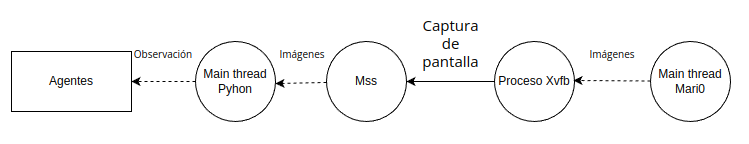
\includegraphics[width=1.0\textwidth]{img/Obsertavions-2.png}
    \caption{Esquema de la alternativa por \textit{Xvfb} [Elaboración Propia]}
    \label{fig:alternativa-2-com}
\end{figure}
\begin{figure}[ht]
    \centering
    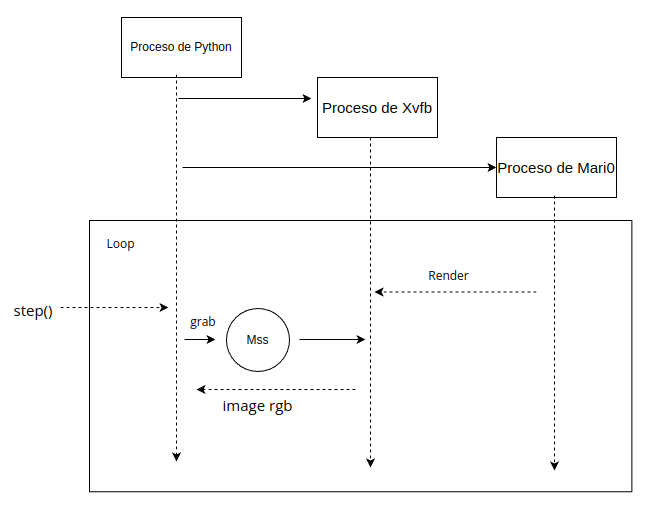
\includegraphics[width=1.0\textwidth]{img/obsevation_sequence.png}
    \caption{Diagrama de secuencia de la alternativa por \textit{Xvfb} [Elaboración Propia]}
    \label{fig:alternativa-2-seq}
\end{figure}

Esta alternativa es mucho más simple que la alternativa por sockets, además, no requiere modificar el sistema de renderizado del videojuego ni tampoco sincronización de threads ni comunicación entre sockets. 

Otra ventaja de esta alternativa es que nos permite observar el funcionamiento del entorno desde 0 e incluso interactuar directamente con el entorno gráfico usando un servidor y cliente de \textit{VNC}. Esto es muy útil para visualizar el entorno y sobre todo para la fase de testing. Cubriremos este proceso en la fase de testing.

Finalmente, implementar la función \textit{Render} de \textit{PettingZoo} sería aparentemente sencillo, ya que solo deberíamos usar captura de pantalla del módulo \textit{Mss} en el módulo \textit{Pygame}.

Por estos motivos, para el sistema de observaciones escogimos la alternativa por \textit{Xvfb}. Aun así, la idea básica de la alternativa por sockets sería usada para el sistema de comunicación entre procesos, que explicaremos más adelante. 

En la siguiente figura podemos ver la implementación de la alternativa por \textit{Xvfb}.

\begin{lstlisting}[language=Python]
    def start_xvfb(self) -> int:
        self.xvfb_process = Xvfb(
            width=SCR_W, height=SCR_H, colordepth=SCR_D * 8)
        self.xvfb_process.start()
        self.status.vdisplay_active = True
        print(f'Using DISPLAY {self.xvfb_process.new_display}')
        return self.xvfb_process.new_display

    def _start_game(self) -> None:
        game_dir = self.config["love_game"]
        env = "env"
        if self.human_player:
            env = "dev"
        else:
            self.display = self.start_xvfb()
        cmd = ["love", game_dir, env]
        self.game_proc = subprocess.Popen(
            cmd, env=os.environ.copy(), shell=False,
            stderr=subprocess.PIPE,)
        time.sleep(3)
        if not self.game_proc.poll(): 
            self.status.game_active = True
        else:
            self.close()
            raise Exception("Game couldn't open")
    def _observe(self):
            offset_x = 0
            offset_y = 0
            if self.human_player:
                offset_x = self.config["offset_x"]
                offset_y = self.config["offset_y"]
            image_array = np.array(self.mss_grabber.grab(
                {"top": offset_y,
                "left": offset_x,
                "width": SCR_W,
                "height": SCR_H}),
            dtype=np.uint8)
            self.pixel_array = np.flip(image_array[:, :, :3], 2)
            return self.pixel_array
\end{lstlisting}

Además de todo lo explicado anteriormente, también implementamos la posibilidad de que un humano pudiera jugar al mismo tiempo que una IA. Para poder lograr esto desactivamos el uso del virtual frame buffer, así el humano podría ver la escena en su monitor. Sin embargo, hay dos pequeñas desventajas. Cuando se use esta opción, el usuario que vaya a jugar deberá calcular la posición de la ventana del juego en su monitor y este también podría controlar el movimiento de los agentes si quisiera. El primer problema se debe a que no es posible saber la posición de la pantalla desde el proceso de \textit{Python}. Y el segundo se debe a que el usuario podría usar las teclas asignadas al movimiento de otros jugadores y así controlar el movimiento del jugador asignado a la IA.


\subsubsection*{Problemas encontrados}

Realizando la implementación de las observaciones nos encontramos con varios problemas. En esta sección explicaremos brevemente los problemas que tuvimos y su solución.

\begin{itemize}
    \item Conseguir que el proceso de \textit{Mari0} usase el virtual frame buffer en vez de la pantalla. Para esto, es necesario cambiar la variable de entorno del sistema 'display'. Una vez cambiada y creado el proceso es necesario resetearla de fábrica, puesto que podría ocasionar problemas al iniciar otros procesos.
    \item Conseguir que el módulo de \textit{Pygame} renderizara el contenido de la captura de pantalla. Para conseguir esto tuvimos que adaptar el contenido de la captura de pantalla, que venía en formato BRGA a formato RGB.
    \item Si el programa de \textit{Python} se cierra de forma abrupta, es posible que el proceso de \textit{Mari0} y de \textit{Xvfb} queden zombis en el sistema. Este problema no se pudo solucionar directamente, puesto que no podemos controlar cuando el programa se abortará. La única solución es acabar el programa manualmente usando la consola de Linux.
\end{itemize}



